\documentclass[12pt]{article}
\usepackage[letterpaper, margin=1in, headheight=105pt]{geometry}
\usepackage{subcaption}
\usepackage{graphicx}
\usepackage{hyperref}
\usepackage{amssymb}
\usepackage{comment}
\usepackage{minted}
\usemintedstyle{manni}



\begin{document}
\setcounter{section}{1}
\tableofcontents
\newpage
\begin{comment}
\section{Homework \thesection\ Report}

\newpage
\subsection{Layers}
\begin{scriptsize}
\inputminted[frame=single,framesep=10pt,linenos, breaklines,xleftmargin=\parindent,xrightmargin=\parindent]{python}{./Homework1/code/layers.py}
\end{scriptsize}


\newpage
\subsection{Logistic}
\subsubsection{Implementation}
\begin{scriptsize}
\inputminted[frame=single,framesep=10pt,linenos, breaklines,xleftmargin=\parindent,xrightmargin=\parindent]{python}{./Homework1/code/logistic.py}
\end{scriptsize}

\newpage
\subsubsection{Simple logistic classifier}
\inputminted[frame=single,framesep=10pt,linenos, breaklines,xleftmargin=\parindent,xrightmargin=\parindent]{python}{./Homework1/code/logistic1.out}

\newpage
\subsubsection{2-layer neural network with logistic regression}
\inputminted[frame=single,framesep=10pt,linenos, breaklines,xleftmargin=\parindent,xrightmargin=\parindent]{python}{./Homework1/code/logistic2.out}


\newpage
\subsection{Support vector machine}
\subsubsection{Implementation}
\begin{scriptsize}
\inputminted[frame=single,framesep=10pt,linenos, breaklines,xleftmargin=\parindent,xrightmargin=\parindent]{python}{./Homework1/code/svm.py}
\end{scriptsize}

\newpage
\subsubsection{Binary SVM classifier}
\inputminted[frame=single,framesep=10pt,linenos, breaklines,xleftmargin=\parindent,xrightmargin=\parindent]{python}{./Homework1/code/svm1.out}

\newpage
\subsubsection{2-lay neural network with hinge loss}
\inputminted[frame=single,framesep=10pt,linenos, breaklines,xleftmargin=\parindent,xrightmargin=\parindent]{python}{./Homework1/code/svm2.out}

\newpage
\subsection{Softmax}
\subsubsection{Implementation}
\begin{scriptsize}
\inputminted[frame=single,framesep=10pt,linenos, breaklines,xleftmargin=\parindent,xrightmargin=\parindent]{python}{./Homework1/code/softmax.py}
\end{scriptsize}

\newpage
\subsubsection{Softmax multi-class classifier}
\inputminted[frame=single,framesep=10pt,linenos, breaklines,xleftmargin=\parindent,xrightmargin=\parindent]{python}{./Homework1/code/softmax1.out}

\newpage
\subsubsection{2-layer neural network with softmax loss}
\inputminted[frame=single,framesep=10pt,linenos, breaklines,xleftmargin=\parindent,xrightmargin=\parindent]{python}{./Homework1/code/softmax2.out}

\newpage
\subsection{Convolutional neural network}
\subsubsection{Implementation}
\begin{scriptsize}
\inputminted[frame=single,framesep=10pt,linenos, breaklines,xleftmargin=\parindent,xrightmargin=\parindent]{python}{./Homework1/code/cnn.py}
\end{scriptsize}


\subsubsection{CNN multi-class classifier}
I am not able to train CNN.

\newpage
\subsection{Convolutional neural network}
\subsubsection{Implementation}
\begin{scriptsize}
\inputminted[frame=single,framesep=10pt,linenos, breaklines,xleftmargin=\parindent,xrightmargin=\parindent]{python}{./Homework1/code/vgg.py}
\end{scriptsize}

\newpage
\subsubsection{Test}
\inputminted[frame=single,framesep=10pt,linenos, breaklines,xleftmargin=\parindent,xrightmargin=\parindent]{python}{./Homework1/code/vgg.out}
\subsubsection{Different optimizer}
The accuracy does not significantly improve by changing the optimizer and learning rate strategy.


\newpage
\subsection{Short answer questions}

\subsubsection{Sigmoid non-linearity}
Sigmoid brings issues when the number of layers increases because the derivative terms that are less than 1 will be multiplied each other many times that the values will become smaller and smaller until the gradient will vanish.

\subsubsection{Training loss}
I may decrease the learning rate.
\end{comment}


\section{Homework \thesection\ Report}
\subsection{Transfer learning}
\begin{tiny}
\inputminted[frame=single,framesep=10pt,linenos, breaklines,xleftmargin=\parindent,xrightmargin=\parindent]{python}{./Homework2/code/transfer_learning.py}
\end{tiny}
\begin{figure}[htbp]
    \centering
    \begin{subfigure}[t]{0.48\textwidth}
        \centering
        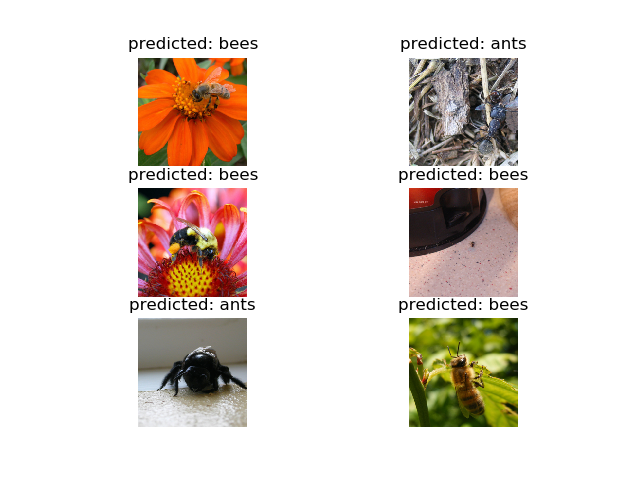
\includegraphics[trim={3in 0in 3in 0in},scale=0.8]{./Homework2/output/hw2p1_fig01.png}
        \caption{Test 1}
    \label{hw2p1a}
    \end{subfigure}\\
    \begin{subfigure}[t]{0.48\textwidth}
        \centering
        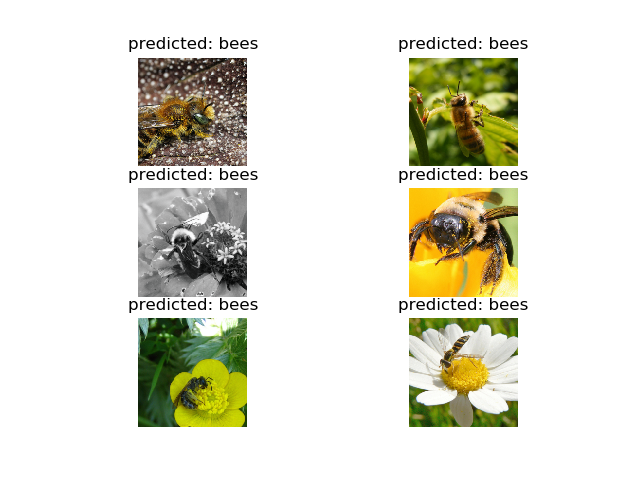
\includegraphics[trim={3in 0in 3in 0in},scale=0.8]{./Homework2/output/hw2p1_fig02.png}
        \caption{Test 2}
    \label{hw2p1b}
    \end{subfigure}
    \caption{Transfer learning}
\end{figure}

\newpage
\subsection{Style Transfer}
\begin{tiny}
\inputminted[frame=single,framesep=10pt,linenos, breaklines,xleftmargin=\parindent,xrightmargin=\parindent]{python}{./Homework2/code/style_transfer.py}
\end{tiny}
\begin{figure}[htbp]
    \centering
    \begin{subfigure}[t]{0.48\textwidth}
        \centering
        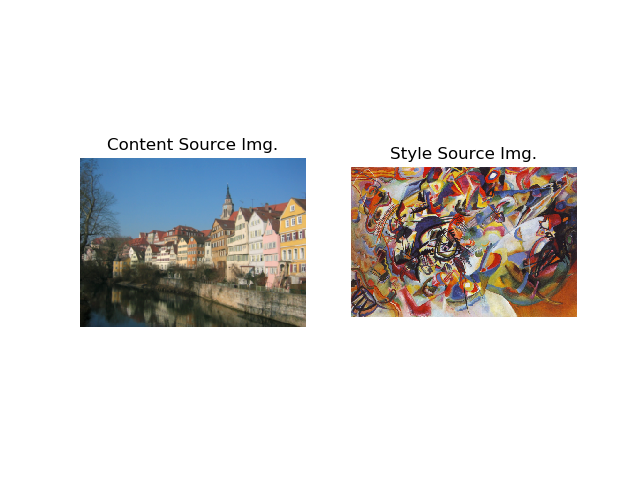
\includegraphics[trim={3in 1in 3in 2in},scale=0.8]{./Homework2/output/hw2p2_fig01.png}
        \caption{Content and Source}
    \label{hw2p2a}
    \end{subfigure}\\
    \begin{subfigure}[t]{0.48\textwidth}
        \centering
        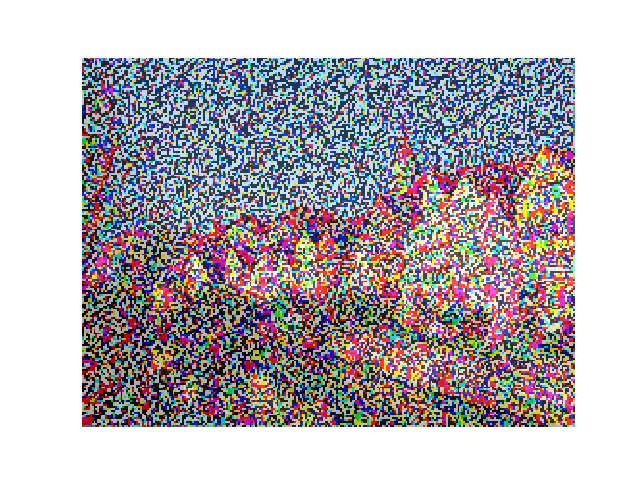
\includegraphics[trim={3in 0in 3in 0in},scale=0.5]{./Homework2/output/hw2p2_fig02.png}
        \caption{Iteration 0}
    \label{hw2p2b}
    \end{subfigure}
    \begin{subfigure}[t]{0.48\textwidth}
        \centering
        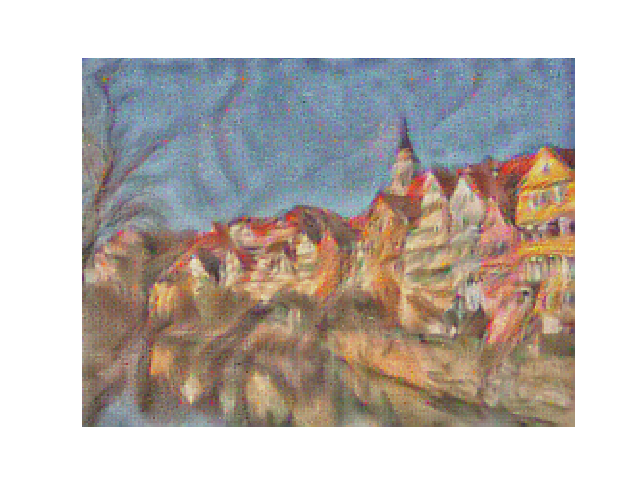
\includegraphics[trim={3in 0in 3in 0in},scale=0.5]{./Homework2/output/hw2p2_fig03.png}
        \caption{Iteration 100}
    \label{hw2p2c}
    \end{subfigure}
    \begin{subfigure}[t]{0.48\textwidth}
        \centering
        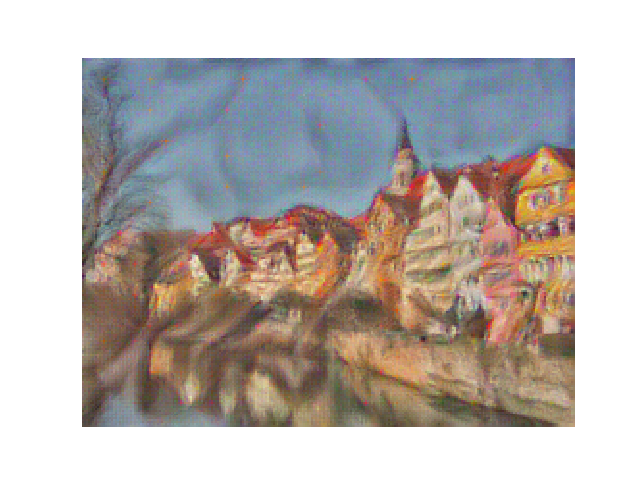
\includegraphics[trim={3in 0in 3in 0in},scale=0.8]{./Homework2/output/hw2p2_fig04.png}
        \caption{Iteration 200}
    \label{hw2p2d}
    \end{subfigure}
    \caption{Style transfer for Tubingen \& Composition VII}
\end{figure}


\begin{figure}[htbp]
    \centering
    \begin{subfigure}[t]{0.48\textwidth}
        \centering
        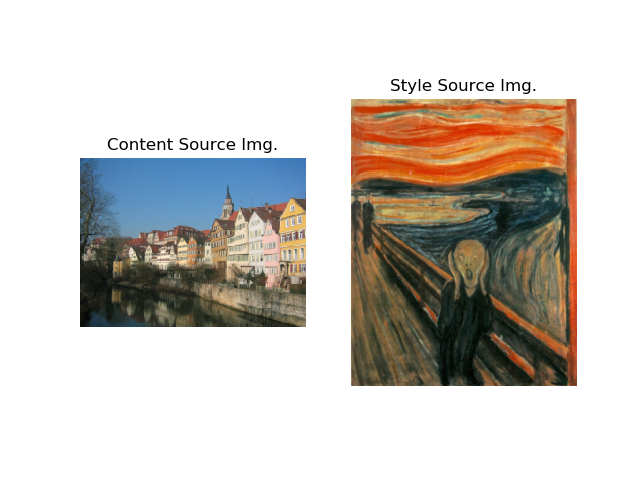
\includegraphics[trim={3in 1in 3in 1in},scale=0.8]{./Homework2/output/hw2p2_fig05.png}
        \caption{Content and Source}
    \label{hw2p2e}
    \end{subfigure}\\
    \begin{subfigure}[t]{0.48\textwidth}
        \centering
        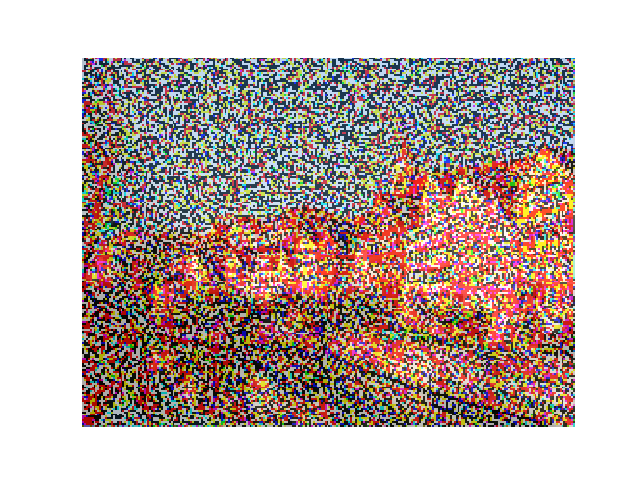
\includegraphics[trim={3in 0in 3in 0in},scale=0.45]{./Homework2/output/hw2p2_fig06.png}
        \caption{Iteration 0}
    \label{hw2p2f}
    \end{subfigure}
    \begin{subfigure}[t]{0.48\textwidth}
        \centering
        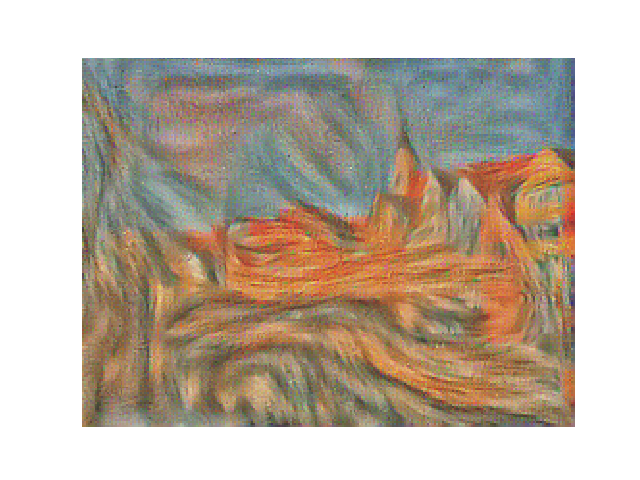
\includegraphics[trim={3in 0in 3in 0in},scale=0.45]{./Homework2/output/hw2p2_fig07.png}
        \caption{Iteration 100}
    \label{hw2p2g}
    \end{subfigure}
    \begin{subfigure}[t]{0.48\textwidth}
        \centering
        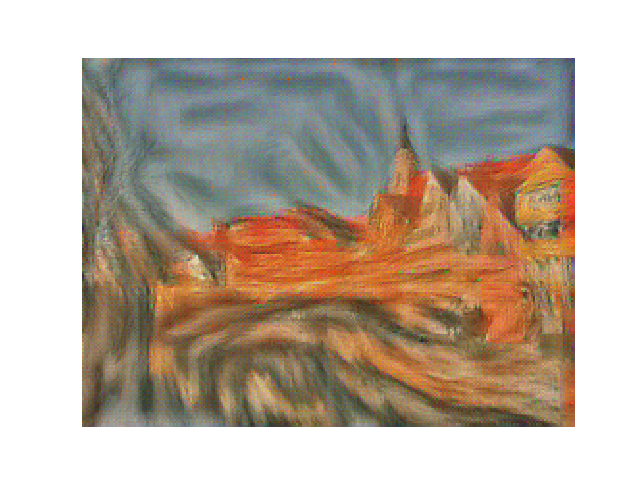
\includegraphics[trim={3in 0in 3in 0in},scale=0.7]{./Homework2/output/hw2p2_fig08.png}
        \caption{Iteration 200}
    \label{hw2p2h}
    \end{subfigure}
    \caption{Style transfer for Tubingen \& The Scream}
\end{figure}


\begin{figure}[htbp]
    \centering
    \begin{subfigure}[t]{0.48\textwidth}
        \centering
        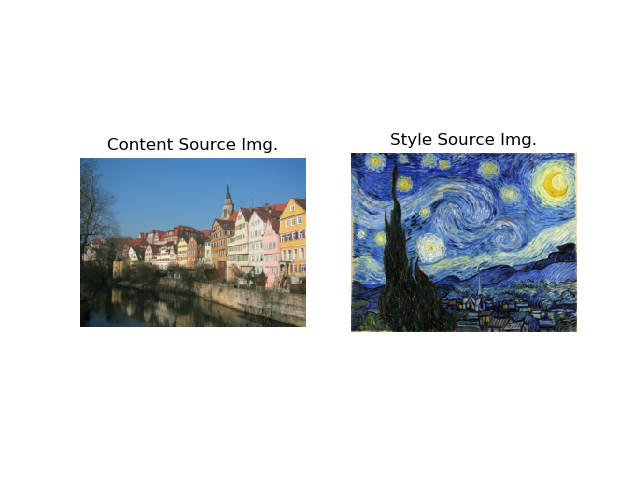
\includegraphics[trim={3in 1in 3in 1in},scale=0.8]{./Homework2/output/hw2p2_fig09.png}
        \caption{Content and Source}
    \label{hw2p2i}
    \end{subfigure}\\
    \begin{subfigure}[t]{0.48\textwidth}
        \centering
        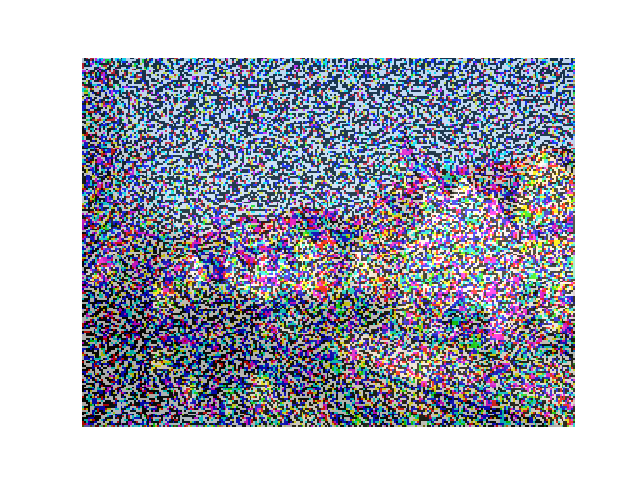
\includegraphics[trim={3in 0in 3in 0in},scale=0.45]{./Homework2/output/hw2p2_fig10.png}
        \caption{Iteration 0}
    \label{hw2p2j}
    \end{subfigure}
    \begin{subfigure}[t]{0.48\textwidth}
        \centering
        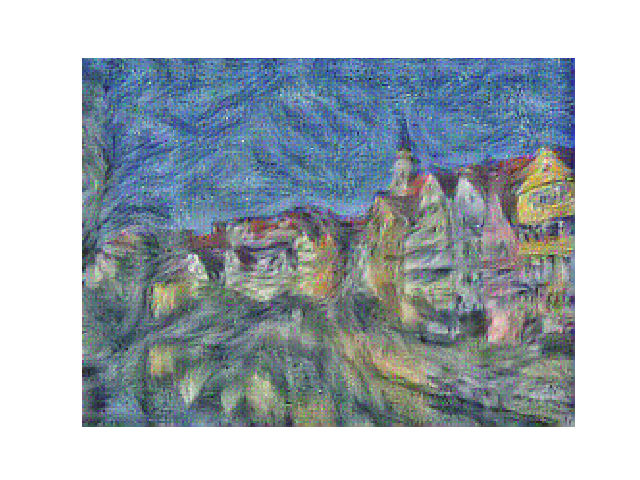
\includegraphics[trim={3in 0in 3in 0in},scale=0.45]{./Homework2/output/hw2p2_fig11.png}
        \caption{Iteration 100}
    \label{hw2p2k}
    \end{subfigure}
    \begin{subfigure}[t]{0.48\textwidth}
        \centering
        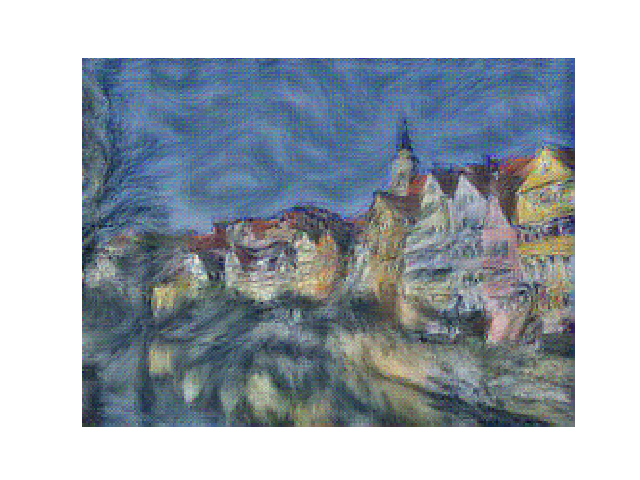
\includegraphics[trim={3in 0in 3in 0in},scale=0.7]{./Homework2/output/hw2p2_fig12.png}
        \caption{Iteration 200}
    \label{hw2p2l}
    \end{subfigure}
    \caption{Style transfer for Tubingen \& Starry Night}
\end{figure}

\subsection{Forward and Backward propagation module for RNN}

\subsection{Forward and Backward propagation module for LSTM}

\subsection{Application to Image Captioning}
\begin{figure}[htbp]
    \centering
    \begin{subfigure}[t]{0.48\textwidth}
        \centering
        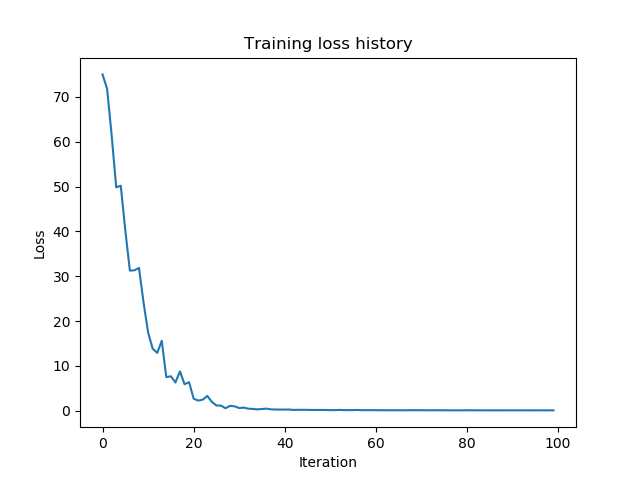
\includegraphics[trim={3in 0in 3in 1in},scale=0.7]{./Homework2/output/hw2p5_fig01.png}
        \caption{Learning curve}
    \label{hw2p5a}
    \end{subfigure}\\
    \begin{subfigure}[t]{0.48\textwidth}
        \centering
        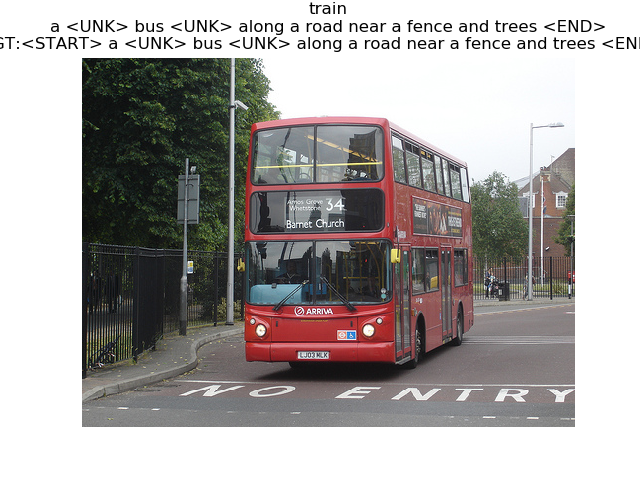
\includegraphics[trim={3in 0in 3in 0in},scale=0.5]{./Homework2/output/hw2p5_fig02.png}
        \caption{Train}
    \label{hw2p5b}
    \end{subfigure}
    \begin{subfigure}[t]{0.48\textwidth}
        \centering
        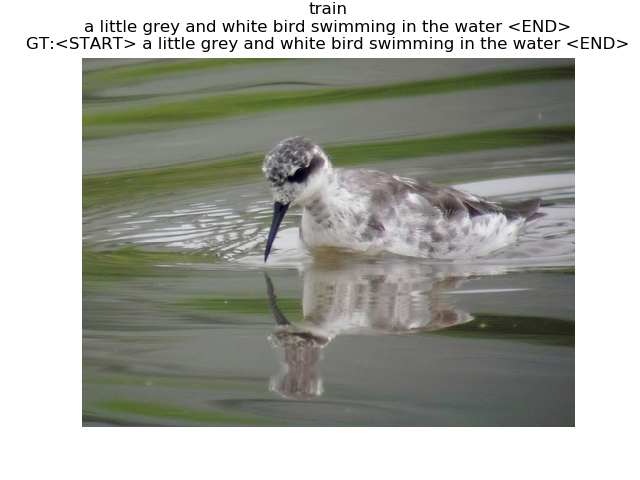
\includegraphics[trim={3in 0in 3in 0in},scale=0.5]{./Homework2/output/hw2p5_fig03.png}
        \caption{Train}
    \label{hw2p5c}
    \end{subfigure}
    \begin{subfigure}[t]{0.48\textwidth}
        \centering
        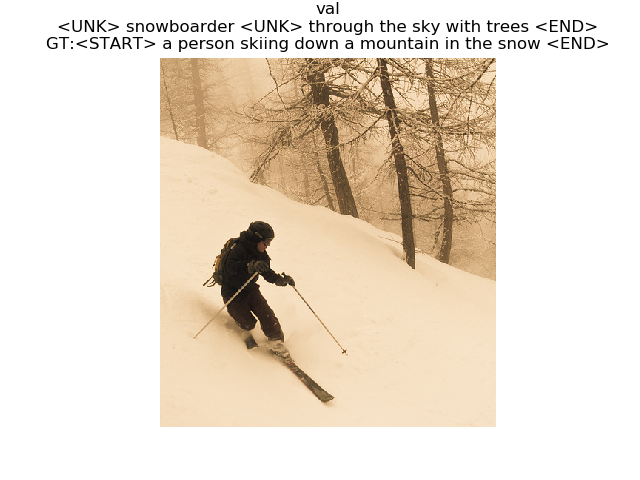
\includegraphics[trim={3in 0in 3in 0in},scale=0.5]{./Homework2/output/hw2p5_fig04.png}
        \caption{Val}
    \label{hw2p5d}
    \end{subfigure}
    \begin{subfigure}[t]{0.48\textwidth}
        \centering
        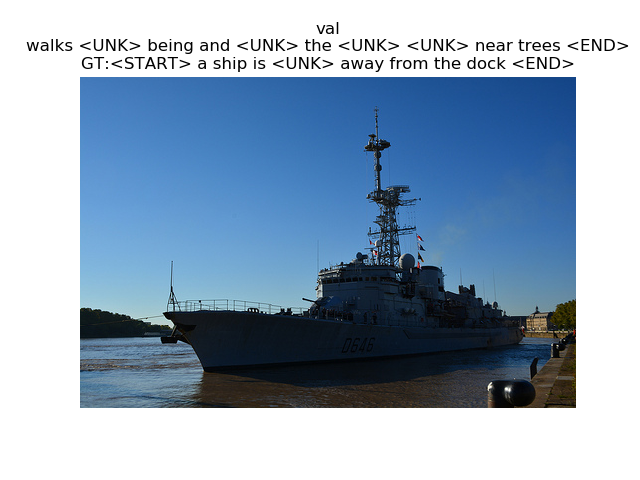
\includegraphics[trim={3in 0in 3in 0in},scale=0.5]{./Homework2/output/hw2p5_fig05.png}
        \caption{Val}
    \label{hw2p5e}
    \end{subfigure}
    \caption{Image captioning RNN}
\end{figure}
\begin{figure}[htbp]
    \centering
    \begin{subfigure}[t]{0.48\textwidth}
        \centering
        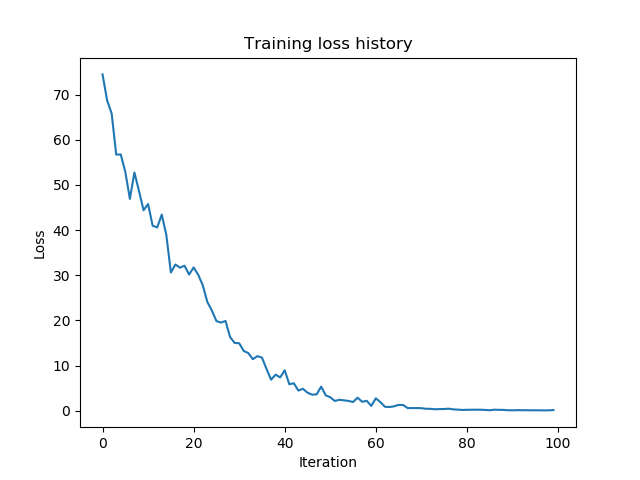
\includegraphics[trim={3in 0in 3in 1in},scale=0.7]{./Homework2/output/hw2p5_fig06.png}
        \caption{Learning curve}
    \label{hw2p5f}
    \end{subfigure}\\
    \begin{subfigure}[t]{0.48\textwidth}
        \centering
        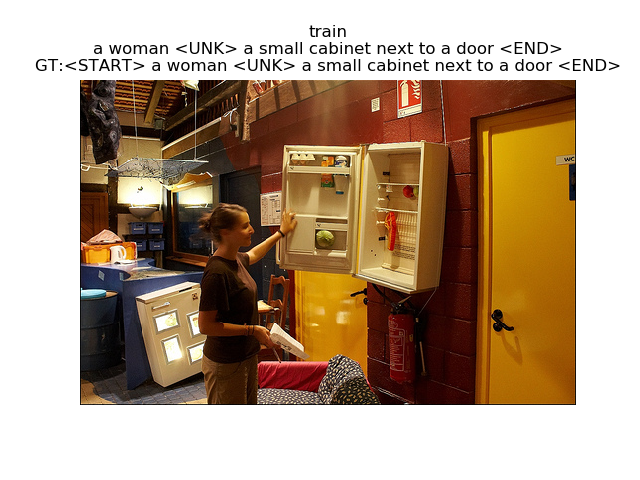
\includegraphics[trim={3in 0in 3in 0in},scale=0.5]{./Homework2/output/hw2p5_fig07.png}
        \caption{Train}
    \label{hw2p5g}
    \end{subfigure}
    \begin{subfigure}[t]{0.48\textwidth}
        \centering
        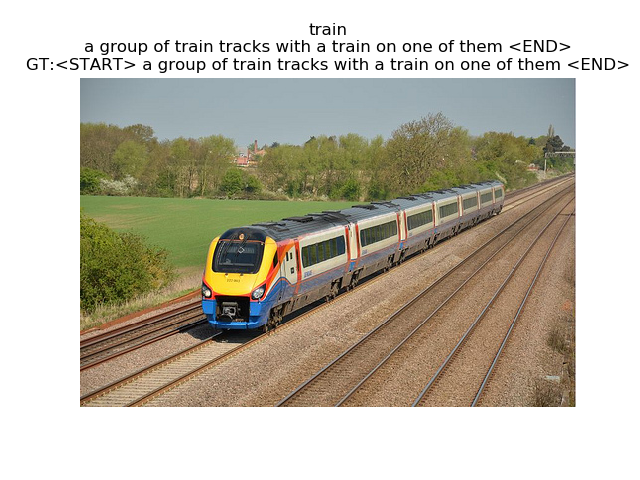
\includegraphics[trim={3in 0in 3in 0in},scale=0.5]{./Homework2/output/hw2p5_fig08.png}
        \caption{Train}
    \label{hw2p5h}
    \end{subfigure}
    \begin{subfigure}[t]{0.48\textwidth}
        \centering
        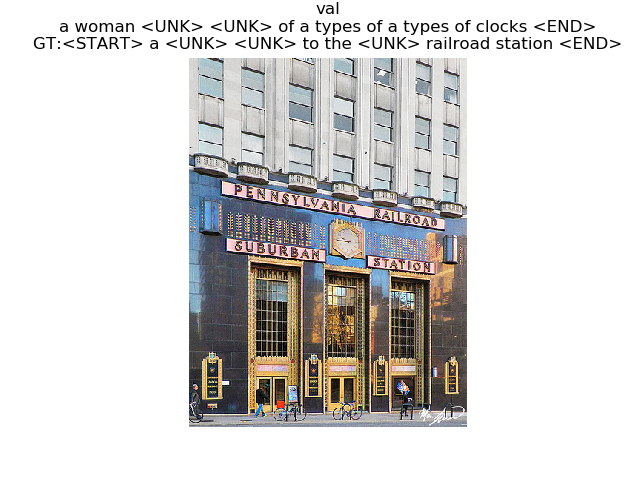
\includegraphics[trim={3in 0in 3in 0in},scale=0.5]{./Homework2/output/hw2p5_fig09.png}
        \caption{Val}
    \label{hw2p5i}
    \end{subfigure}
    \begin{subfigure}[t]{0.48\textwidth}
        \centering
        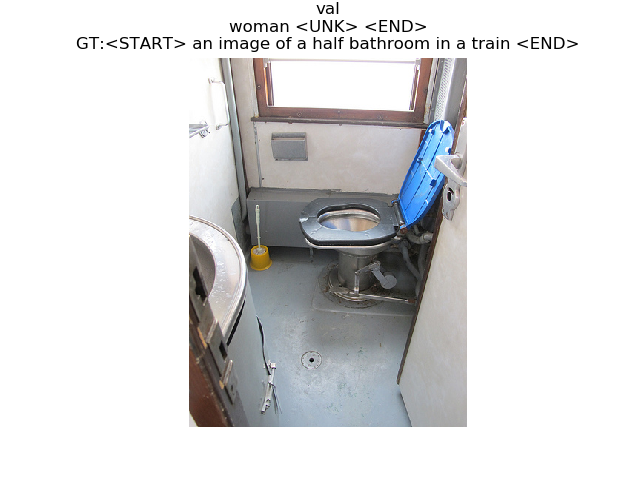
\includegraphics[trim={3in 0in 3in 0in},scale=0.5]{./Homework2/output/hw2p5_fig10.png}
        \caption{Val}
    \label{hw2p5j}
    \end{subfigure}
    \caption{Image captioning RNN}
\end{figure}

\subsection{Application to text classification}

\end{document}